\chapter{Materiais utilizados}
\label{chap:materiais}

As ferramentas de desenvolvimento do navegador, também conhecidas como \textit{DevTools}, são conjuntos de ferramentas incorporadas nos navegadores da web, como Google Chrome e Mozilla Firefox. Essas ferramentas permitem que os desenvolvedores da web inspecionem e depurem o código-fonte da página, além de analisar o desempenho, uso de memória de seus aplicativos da web, entre outros recursos \cite{apple}. Durante o desenvolvimento deste trabalho foram utilizadas as ferramentas listadas abaixo.

\section{Chrome DevTools}
O Chrome DevTools, Figura \ref{fig:chrome-devtools}, representam um conjunto abrangente de ferramentas integradas ao navegador Google Chrome, essenciais para o desenvolvimento e depuração de aplicações web. Com ele é possível inspecionar o DOM, analisar o desempenho da página, depurar JavaScript, simular diferentes dispositivos, entre outros recursos. \cite{chrome}.
\begin{figure}[!htb]
    \centering
    \caption{Chrome Devtools}
    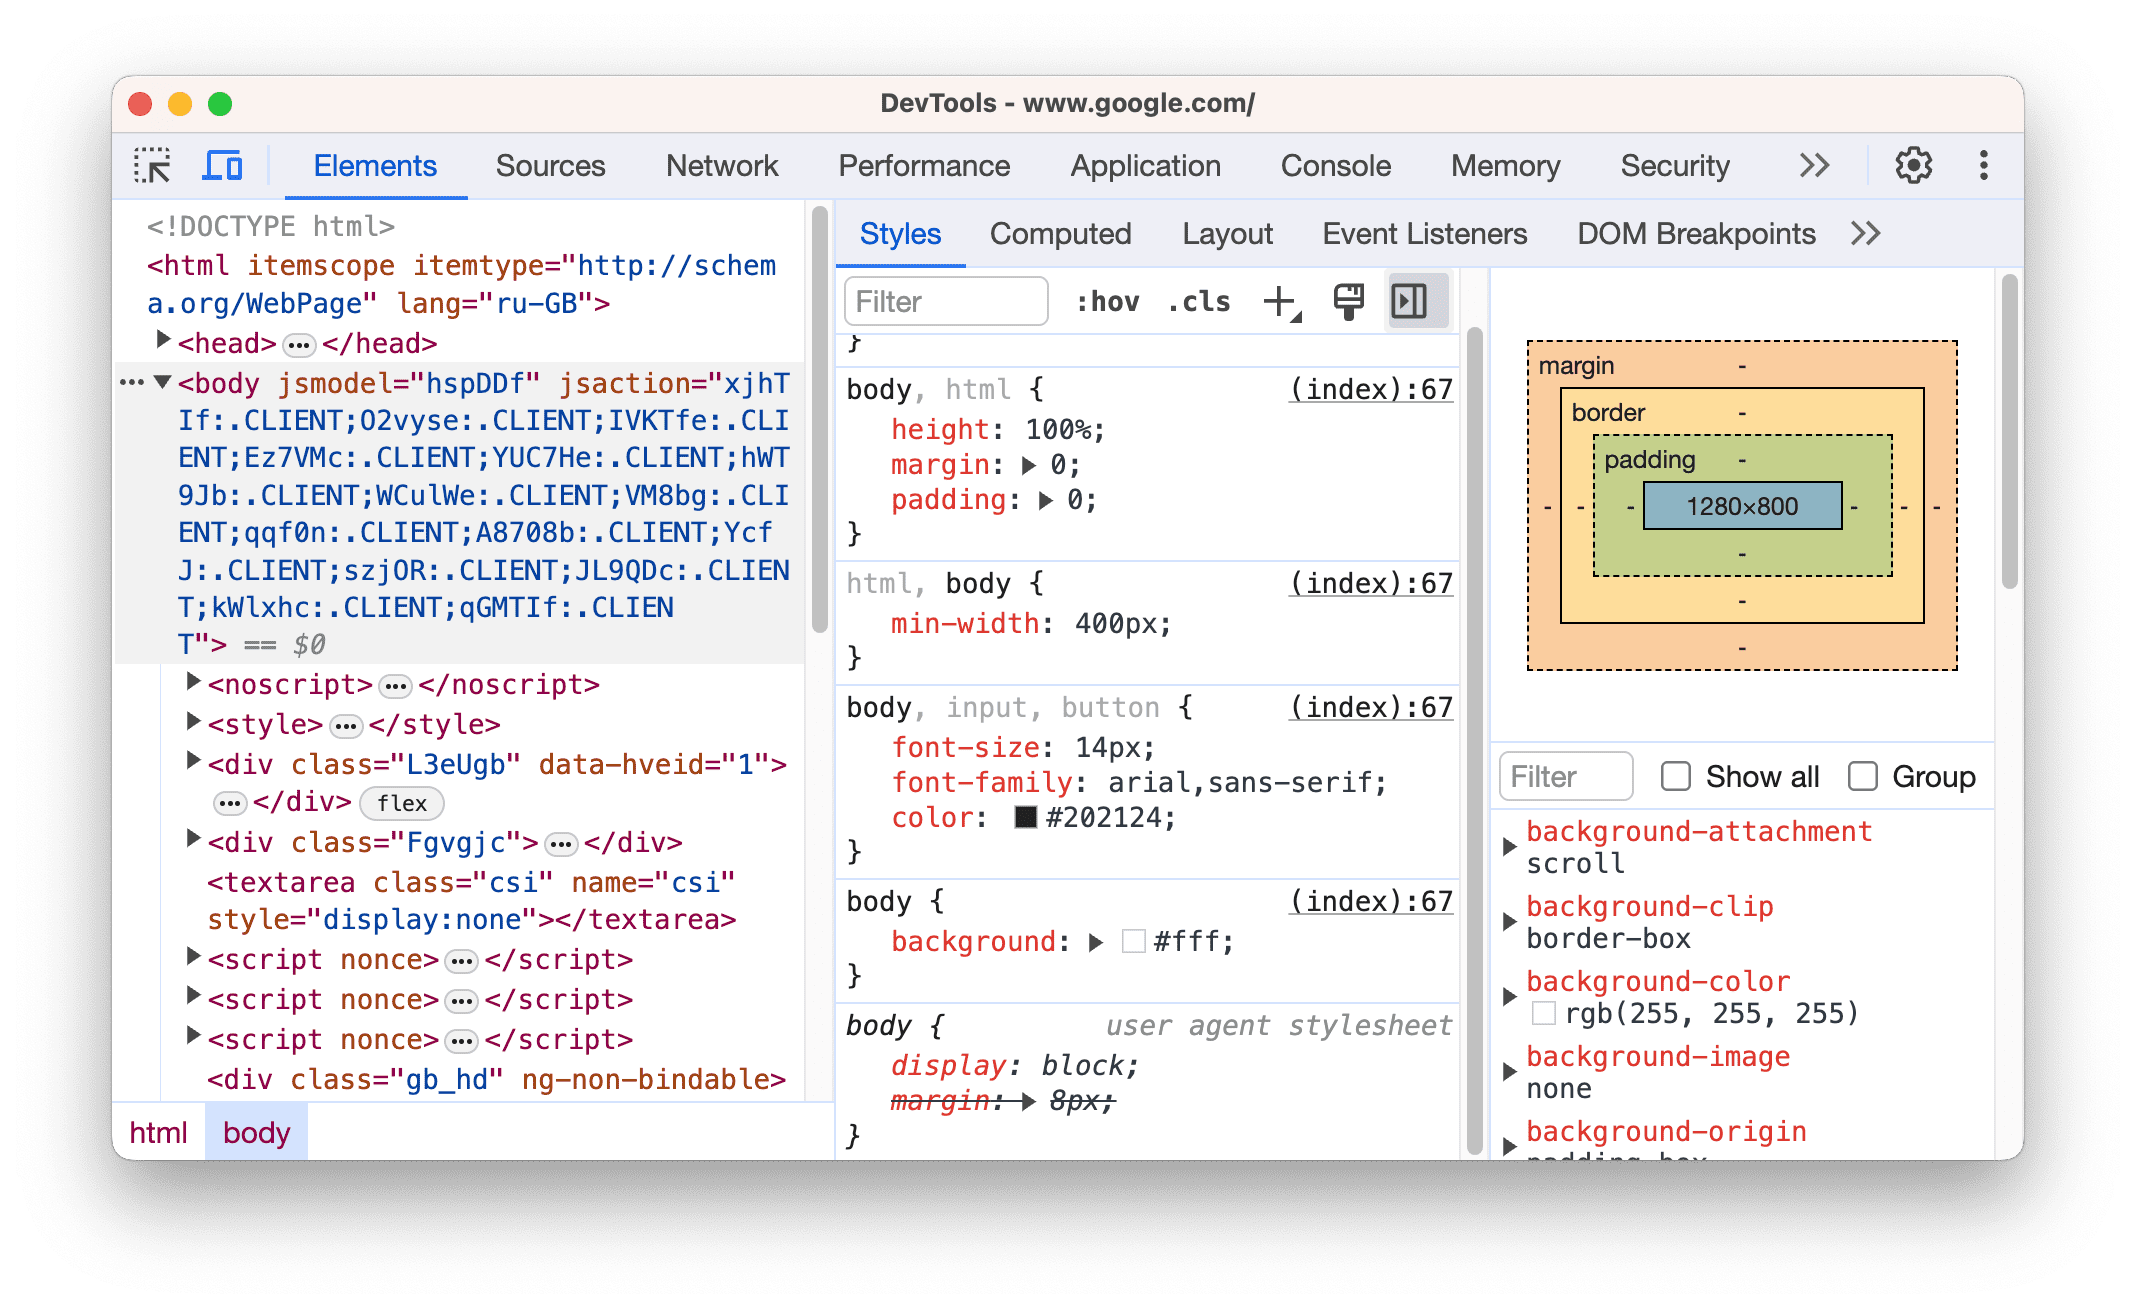
\includegraphics[width=0.65 \linewidth]{assets/chrome-devtools.png}\\
    {\footnotesize Fonte: Chrome for Developers}
    \label{fig:chrome-devtools}
\end{figure}
\newpage
\section{Firefox Developer Tools}
O Firefox Developer Tools, ilustrado na Figura \ref{fig:firefox}, oferece uma alternativa robusta aos Chrome DevTools, com um foco em privacidade e personalização. Essas ferramentas proporcionam um ambiente de desenvolvimento completo, permitindo a inspeção de elementos, a análise de redes, o depurador de JavaScript, a visualização de estilos CSS e a otimização do desempenho. Além disso, o Firefox Developer Tools se integra perfeitamente com outras ferramentas do ecossistema Mozilla, como o editor de código Visual Studio Code, facilitando o fluxo de trabalho dos desenvolvedores \cite{firefox}.
\begin{figure}[!htb]
    \centering
    \caption{Firefox Developer Tools}
    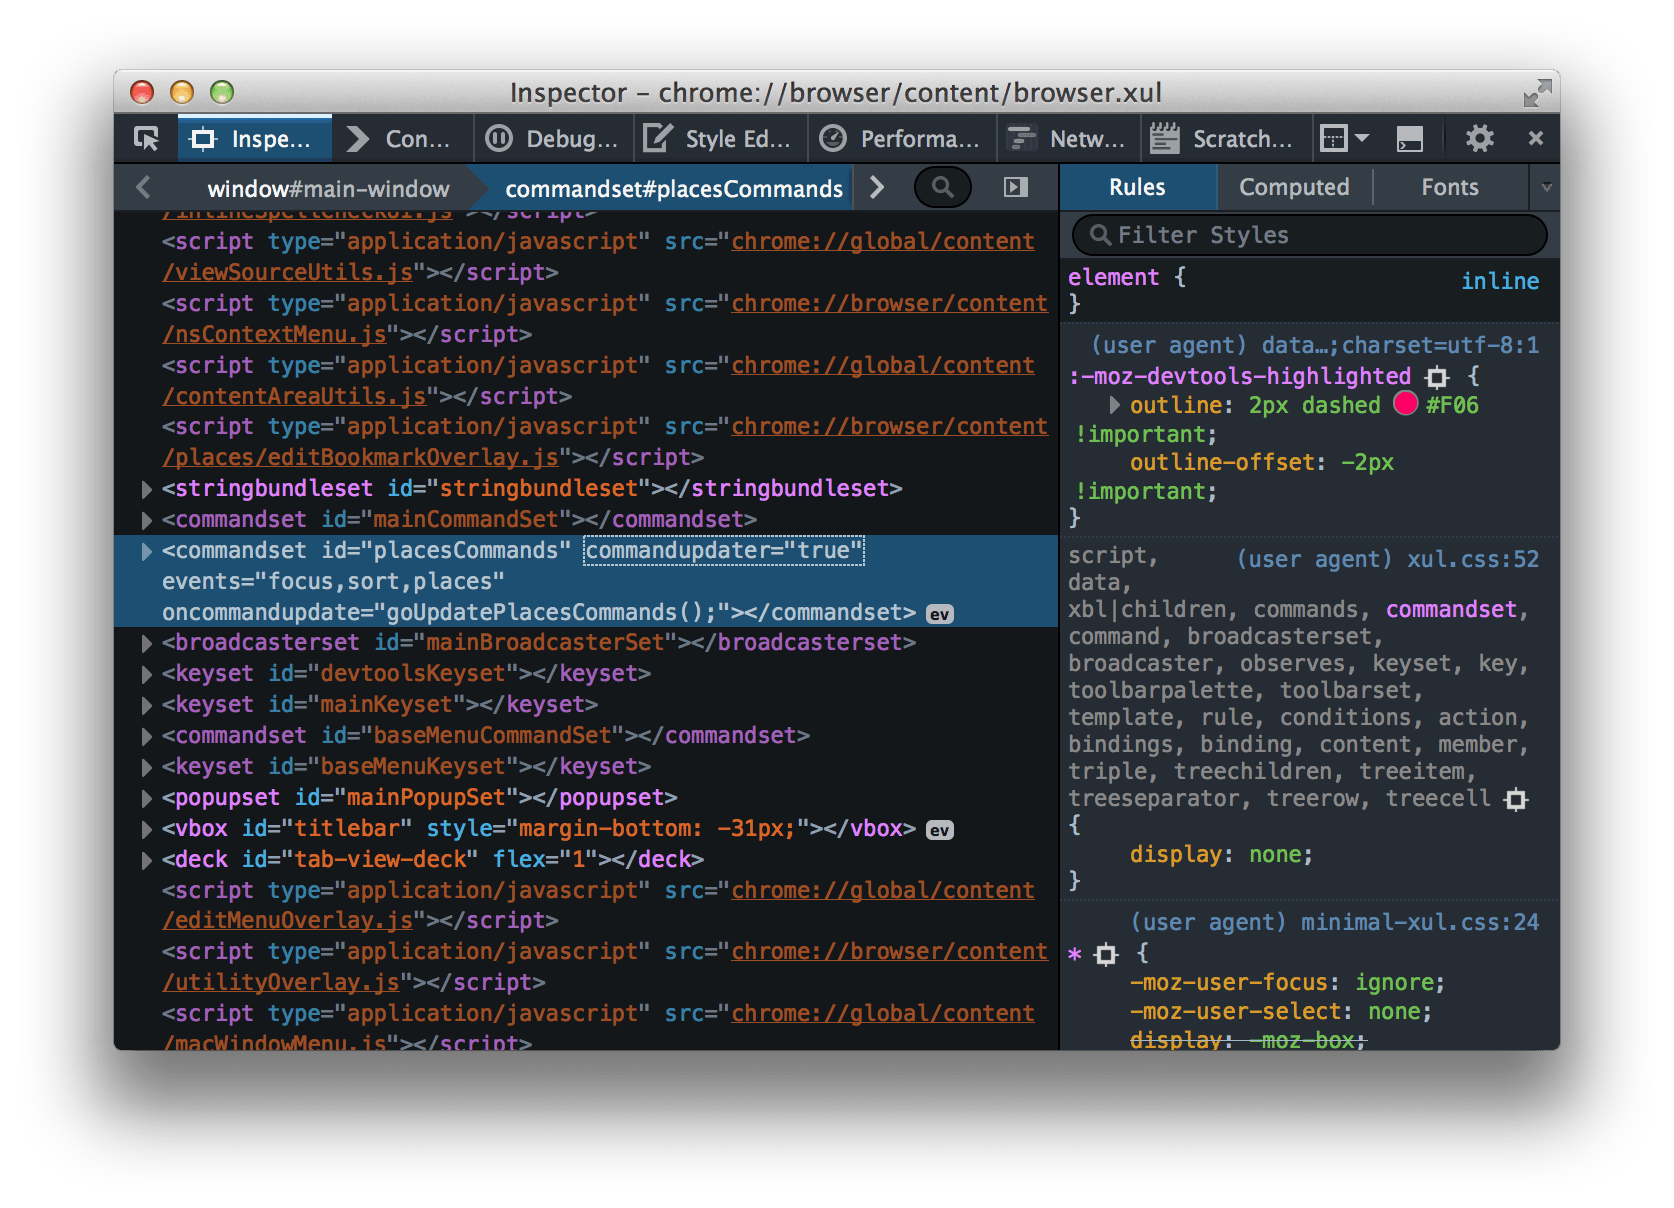
\includegraphics[width=0.8\linewidth]{assets/firefox.png}\\
    {\footnotesize Fonte: Firefox Source Tree Documentation}
    \label{fig:firefox}
\end{figure}
\section{Edge DevTools}
Os Edge DevTools, ilustrado na Figura \ref{fig:edge}, incorporados ao navegador Microsoft Edge, oferecem uma experiência de desenvolvimento moderna e eficiente. Com uma interface visualmente atraente e funcionalidades similares aos Chrome DevTools, os Edge DevTools permitem inspecionar elementos, depurar JavaScript, analisar o desempenho da página e simular diferentes dispositivos. A integração com o Microsoft Visual Studio Code e outras ferramentas do ecossistema Microsoft torna os Edge DevTools uma opção atraente para desenvolvedores que utilizam a plataforma Windows\cite{edge}.

\begin{figure}[!htb]
    \centering
    \caption{Edge DevTools}
    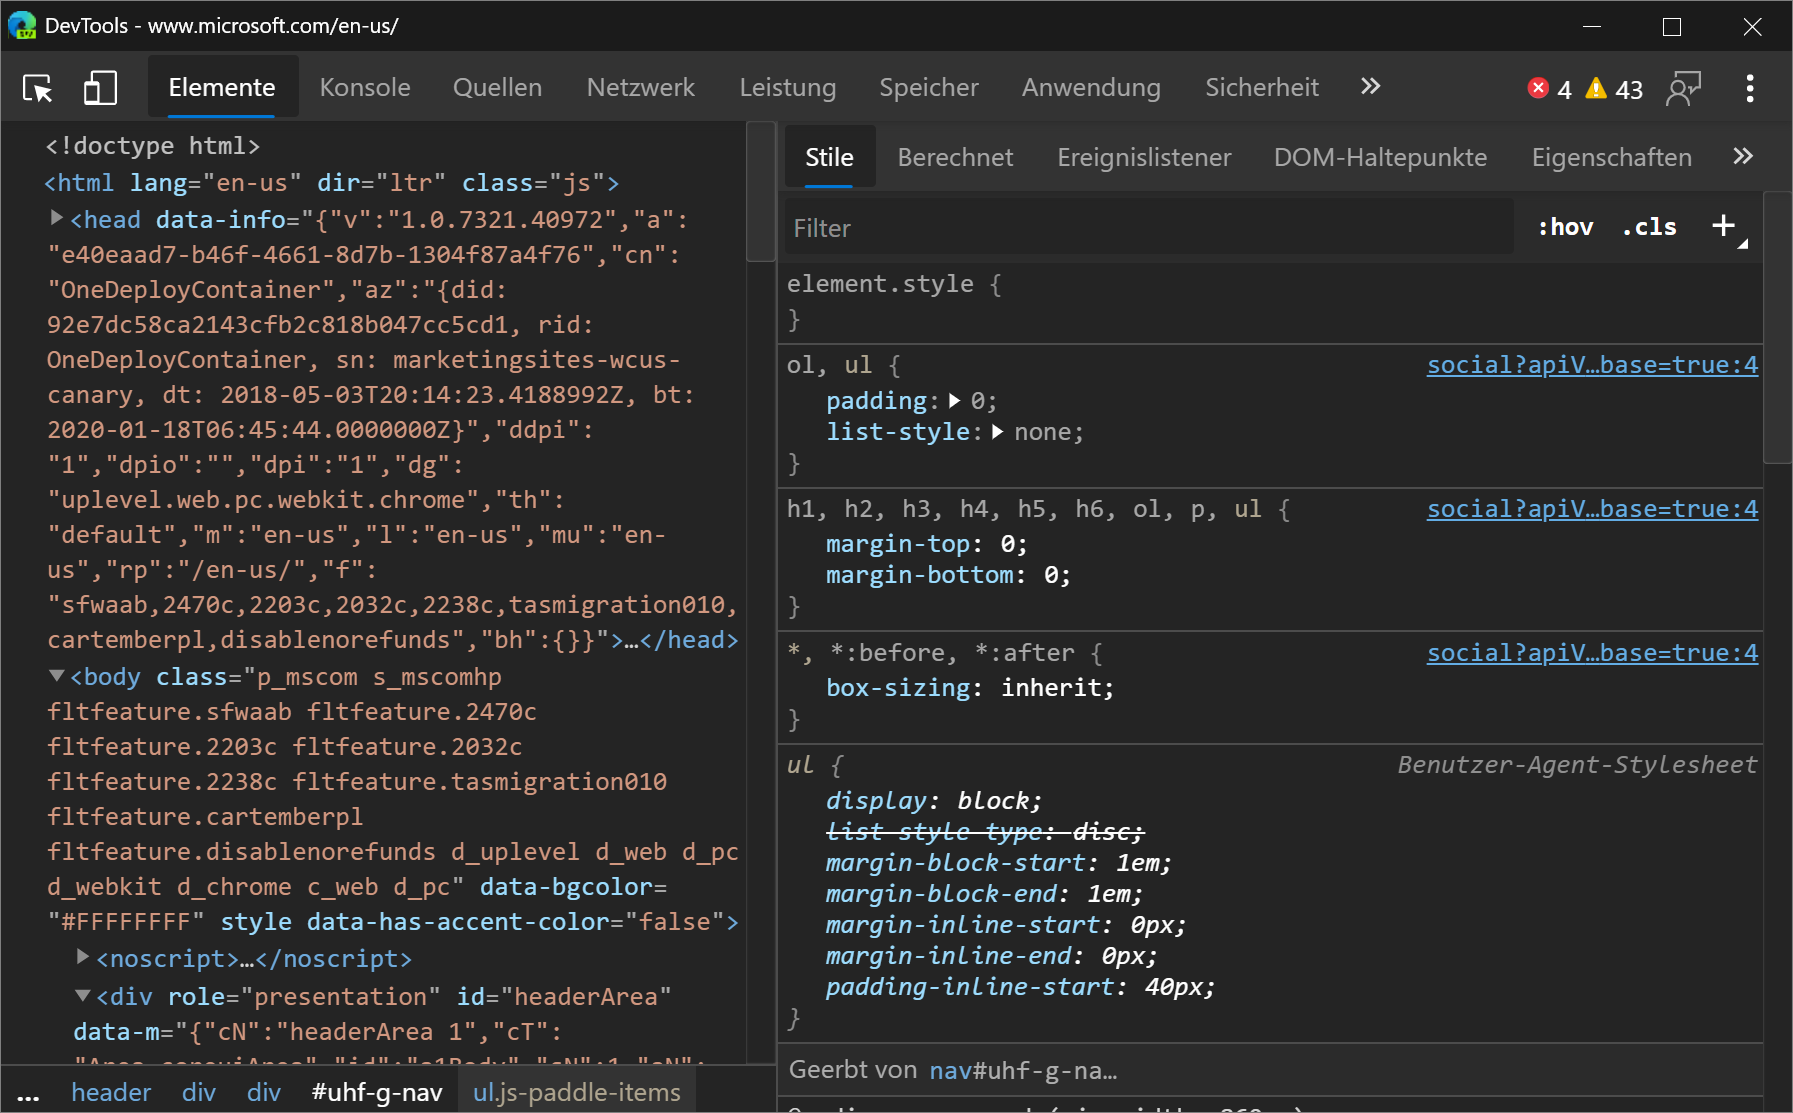
\includegraphics[width=0.8\linewidth]{assets/edge.png}\\
    {\footnotesize Fonte: Microsoft Learn}
    \label{fig:edge}
\end{figure}
\section{Safari Web Inspector}
O Safari Web Inspector, ilustrado na Figura \ref{fig:safari}, é a ferramenta de desenvolvimento integrada ao navegador Apple Safari, projetada para oferecer uma experiência de depuração e desenvolvimento de alta qualidade. Com um foco em desempenho e usabilidade, o Web Inspector permite inspecionar elementos, depurar JavaScript, analisar o desempenho da página e simular diferentes dispositivos\cite{apple}.
\begin{figure}[!htb]
    \centering
    \caption{Safari Web Inspector}
    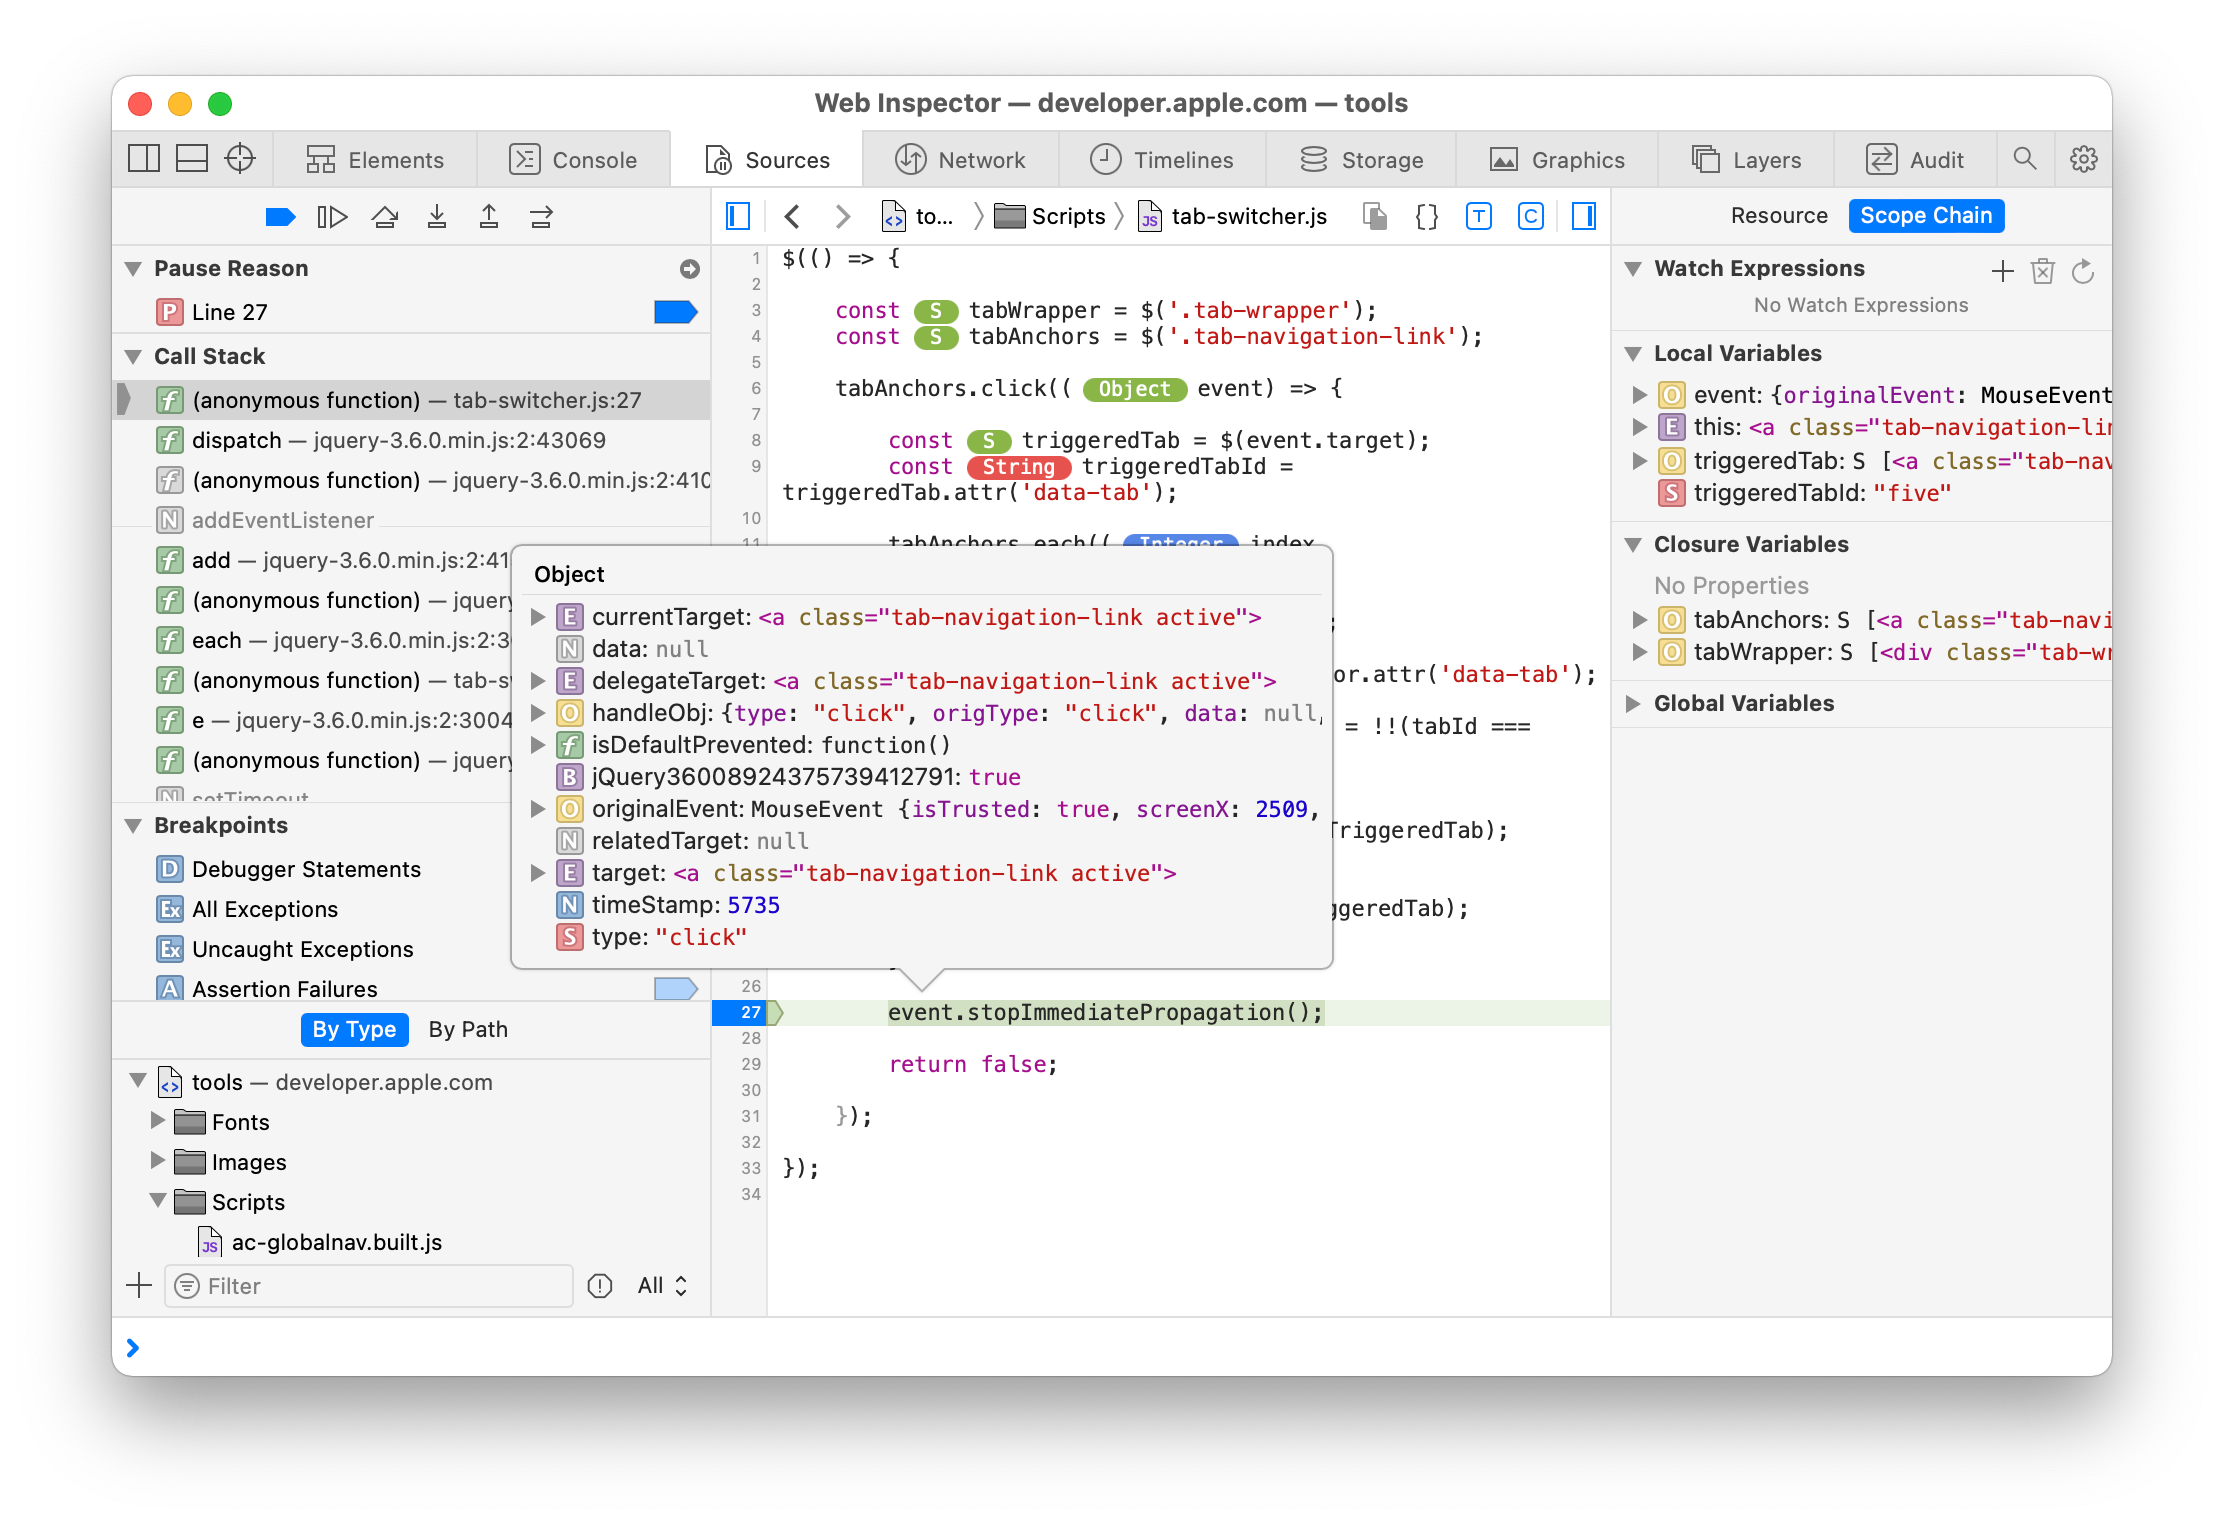
\includegraphics[width=0.8\linewidth]{assets/safari.png}\\
    {\footnotesize Fonte: Apple Developer Documentation}
    \label{fig:safari}
\end{figure}